\chapter{Recherche séquentielle d'un élément dans un tableau}

\section{Description de l'objectif de l'algorithme}
En informatique, un tableau est une structure de données représentant une séquence finie d'éléments définis par un index représentant leurs positions au sein du tableau. C'est un type de conteneur que l'on retrouve dans un grand nombre de langages de programmation et est l'un des plus utilisés dû à sa simplicité.
\par
Les données du tableau étant accessible individuellement il est nécessaire de faire une recherche lorsque l'on souhaite accéder a une valeur spécifique du tableau. Cependant, lorsque la taille de la structure est grande il devient difficile d'y accéder efficacement. Dans ce chapitre nous allons voir la recherche séquentielle qui est une recherche très coûteuse en temps et nous allons aussi présenter une optimisation de cette recherche afin de gagner en complexité temporelle.
\par
La recherche séquentielle ou recherche linéaire est un algorithme pour trouver une valeur dans une liste ou un tableau. Elle consiste simplement à considérer les éléments du tableau les uns après les autres, jusqu'à ce que l'élément soit trouvé, ou que toutes les cases aient été lues. Elle est aussi appelée recherche par balayage. (voir Figure \ref{fig:recherche_sec}).

\begin{figure}[H]
    \centering
        \includegraphics[scale=0.5]{./ressources/Recherche_séquentielle.jpg}
        \caption{Exemple graphique d'une recherche séquentielle}
    \label{fig:recherche_sec}
\end{figure}

\section{Fonctionnement de l'algorithme}
La recherche séquentielle consiste à prendre les éléments du tableau les uns après les autres, jusqu'à avoir trouvé la cible, ou avoir épuisé le tableau.Elle ne demande aucune condition au préalable pour le tableau en entrée; par exemple: il n'est pas necessaire que le tableau soit trié.


\par
Nous pouvons le représenter via le pseudo code suivant :


\begin{function}[H]
    \textbf{Variables :}\\
    i : entier\;
    trouve : bool\;
    \Begin{
        $trouve \leftarrow faux $\;
        $i \leftarrow 0 $\;

         \While{$trouve \leftarrow false \:\: ET \:\: i \: < \: n$}
       {
            
            \If{$tab[i] == valeur$}{
                $trouve \leftarrow vrai $\;
                $i++$\;
            }
        }

            \uIf{$trouve \leftarrow vrai$}{
                $retourner\:\: i-1$\;
            }
            \Else {
             $retourner -1$\;
            }
}
    \caption{sequentielle(Entrée: tab: tableau d'entier; tailleTableau, valeur: entier;)}
\end{function}







\section{Calcul de complexité}
\subsection{Complexité temporelle}
La complexité de la recherche séquentielle est toujours égale à : $\mathcal{O}(n)$.

le tableau suivant représente les temps d'exécution théorique en nanoseconde de l'algorithme selon la variation de la taille de l'expression:

\small
\begin{center}
\begin{tabular}{| c | c | c | c | c | c | c | c | c | c | c | c | c |}
    \hline
    N & 10 & 50 & 100 & 500 & 1000 & 5000 & 10000 & 100000 & 1000000 & 10000000 \\
    \hline
    t(ns) & 10 & 50 & 100 & 500 & 1000 & 5000 & 10000 & 100000 & 1000000 & 10000000 \\
    \hline
\end{tabular}  
\end{center}

La figure suivante (voir Figure \ref{fig:temps_exec_th_algo2}) représente l'évolution du temps d'exécution théorique selon la longueur de l'expression.

\begin{figure}[H]
    \centering
        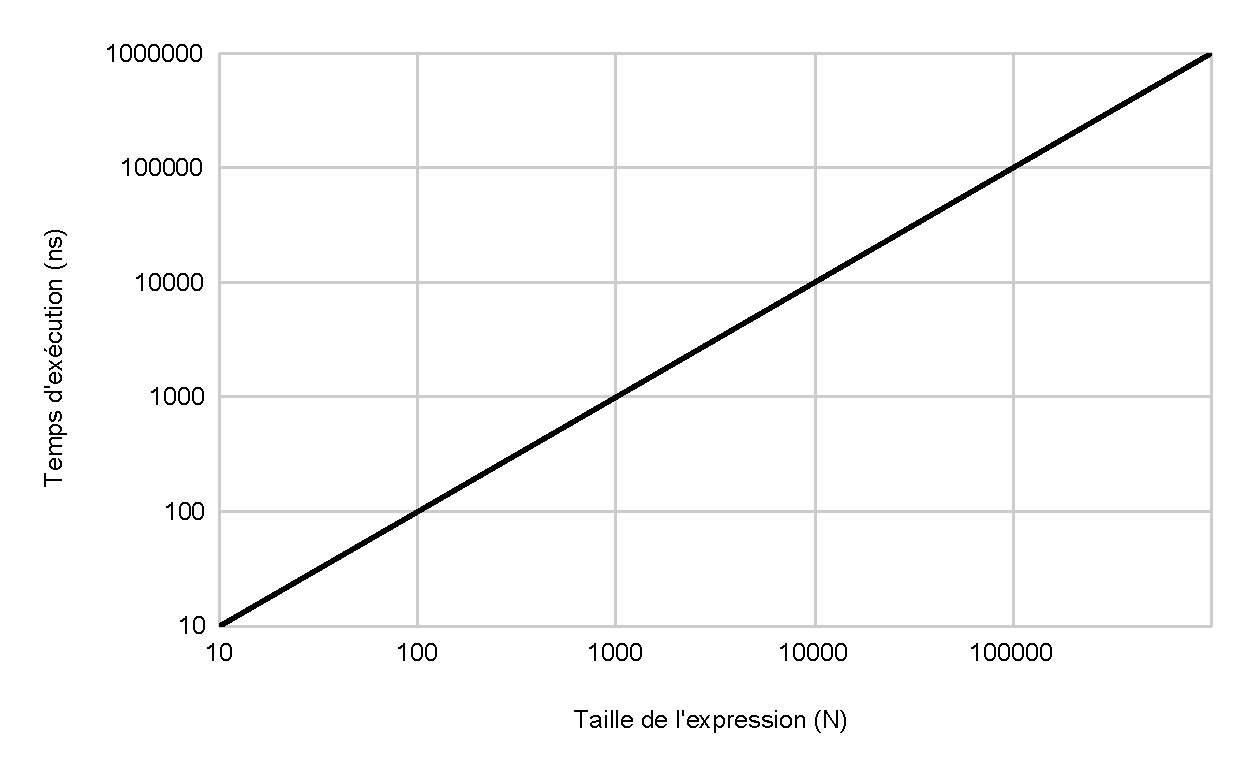
\includegraphics[scale=0.5]{./ressources/temps_execution_th_algo2.pdf}
        \caption{Temps d'exécution théorique de l'algorithme de recherche linéaire}
    \label{fig:temps_exec_th_algo2}
\end{figure} 

Depuis le graphe,  on observe que le temps d'exécution évolue de manière linéaire avec l'évolution de la taille de l'expression.


\subsection{Complexité spatiale}
\par
L'unique structure de données utilisée est un tableau d'entier a n éléments. 
\par
La taille d'un entier étant de 2 octets, la complexité spatiale est donc égale au produit de la taille du tableau et de la taille d'un entier : $n * 2 \approx \mathcal{O}(n)$
\par

\section{Expérimentation}
Le tableau suivant représente les temps d'exécution en nanoseconde de l'algorithme selon la variation de la taille de l'expression arithmétique en d'opérande.\\ \\
\small
\resizebox{19cm}{!}{
\begin{tabular}{| c | c | c | c | c | c | c | c | c | c | c | c | c |}
    \hline
    N &  10 & 50 & 100 & 500 & 1000 & 5000 & 10000 & 100000 & 1000000 & 10000000 \\
    \hline
    t1(ns) & 606 & 401 & 222 & 3224 & 12010 & 6864 & 106408 & 1066370 & 11130 & 11018 \\
    \hline
    t2(ns) & 866 & 1153 & 1851 & 5171 & 11383 & 52809 & 109357 & 1061730 & 3028000 & 38859000 \\
    \hline
    t3(ns) & 168 & 1066 & 1064 & 5714 & 10237 & 53084 & 2875 & 5070 & 4519680 & 56877700 \\
    \hline
    t4(ns) & 744 & 1119 & 1283 & 7111 & 747 & 2197 & 1504 & 11452 & 7636790 & 41331300 \\
    \hline
    t5(ns) & 588 & 785 & 829 & 1328 & 10459 & 3069 & 102717 & 1074940 & 1077270 & 54743600 \\
    \hline
    t6(ns) & 722 & 621 & 1402 & 1556 & 4204 & 10955 & 5509 & 1082590 & 1069420 & 11577 \\
    \hline
    t7(ns) & 638 & 499 & 375 & 5083 & 10259 & 6345 & 106589 & 493002 & 10463 & 38906200 \\
    \hline
    t8(ns) & 708 & 746 & 2192 & 7064 & 5008 & 8755 & 107439 & 1041410 & 1094640 & 40419900 \\
    \hline
    t9(ns) & 694 & 1225 & 1570 & 1118 & 11180  & 3275 & 122386 & 922361 & 10669 & 55940100 \\
    \hline
    t10(ns) & 666 & 1161 & 1504 & 2456 & 11349 & 10799 & 7470 & 1092110 & 7197500 & 40000300 \\
    \hline
    Moyenne(ns) & 582,727273 & 802,3636 & 1126,545 & 3665,909 & 7985,091 & 14832 & 62023,09 & 62023,09 & 2423233 & 34281881,4 \\
    \hline
\end{tabular}}
\\
\normalsize
\par
La figure suivante (voir Figure \ref{fig:temps_exec_seq}) représente l'évolution du temps d'exécution selon la longueur du tableau.

\begin{figure}[H]
    \centering
        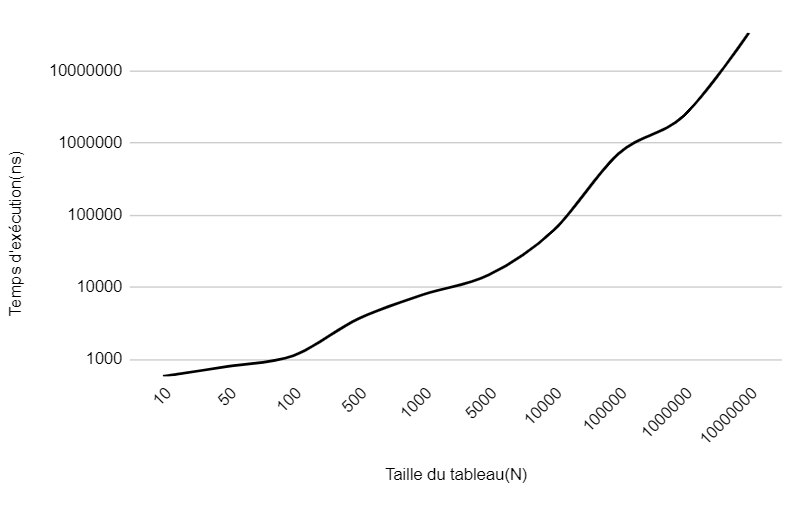
\includegraphics[scale=0.5]{./ressources/graphe_temps_execution.png}
        \caption{Temps d'exécution du programme selon la longueur du tableau}
    \label{fig:temps_exec_seq}
\end{figure}
\par
Depuis le graphe, la courbe est sous forme d'un arc ascendant, on observe que le temps d'exécution évolue de manière presque liénaire avec l'augmentation de la taille du problème, ce qui correspond bien à la complexité théorique calculée auparavant.
On a pas obtenu une droite linéaire car les testes étaient peu et aléatoires.
\section{Amélioration}
L'algorithme de recherche linéaire est coûteux en terme de temps, donc on a pensé à utiliser 2 processus qui vont rechercher la valeur en parallèle pour gagner du temps.
Le premier processus commence à chercher depuis le début jusqu'à la moitié du tableau et le deuxième processus commence de la moitié jusqu'à la fin du tableau. Le premier d'entre eux qui trouve la valeur, il l'envoie au processus père.





\begin{function}[H]
    \textbf{Variables :}\\
    i, pos, status,debut,fin : entier\;
    $pid1, pid2, pid : pid_t$\;
    trouve : bool\;
    
    \Begin{
        $debut  \leftarrow 0$\;
        $fin  \leftarrow  tailleTableau/2 $\;
        $trouve  \leftarrow  faux $\; 
        
        $pid1 = fork()$\;\tcp{on crée le fils 1}
        \uIf {$pid1 == -1$}{
        ecrire("y'a un problème lors de la création du fils 1")\;}
\Else{
\tcp{on commence la recheche du début jusqu'au milieu du tableau}
        \For{$i \leftarrow debut$ \KwTo $fin$}{
             \If{$tab[i] == valeur$}{
                $trouve \leftarrow vrai $\;
                $pos \leftarrow i$\;
            }
        }
\tcp{si le fils 1 trouve la valeur cherchée il affichera sa position sinon il affiche un nombre négatif}
        ecrire(pos)\;
\tcp{si le fils 1 a trouvé la valeur on renvoie sa position sinon on revoie -1}
        exit($f\:\: ?\:\: pos : -1$)\;
    }
    
    $debut \leftarrow tailleTableau/ 2 + 1$\;
    $fin \leftarrow tailleTableau - 1$\;
    
    

    }
    \caption{sequentielleprocessus(Entrée: tab: tableau d'entier tailleTableau, valeur: entier)}
\end{function}

\begin{function}[H]
    \textbf{Variables :}\\
    i, pos, status,debut,fin : entier\;
    $pid1, pid2, pid : pid_t$\;
    trouve : bool\;
    
    \Begin{
     $pid2 = fork()$\;\tcp{on crée le fils 2}
        \uIf {$pid2 == -1$}{
        ecrire("y'a un problème lors de la création du fils 1")\;}
\Else{
\tcp{on commence la recheche du milieu jusqu'à la fin du tableau}
        \For{$i \leftarrow debut$ \KwTo $fin$}{
             \If{$tab[i] == valeur$}{
                $trouve \leftarrow vrai $\;
                $pos \leftarrow i$\;
            }
        }
        ecrire(pos)\;
        exit($f\:\: ?\:\: pos : -1$)\;
    }   
    \While{$(pid = wait(\&status)) != -1$} {
        \tcp{le père attend l'arrivée du premier fils}
       ecrire("on attend le premier fils")\;
    }
       
\uIf {f}{ $retourner \:\: 0$\;}
\Else{
        ecrire ("la valeur cherchée n'existe pas dans le tableau") \;
        $retourner -1$\;
    }
    
    }
    \caption{sequentielleprocessus(Entrée: tab: tableau d'entier tailleTableau, valeur: entier)}
\end{function}

\section{Conclusion}
L'algorithme de la recherche sequentielle(linéaire) se caractérise par son fonctionnement inconditionnel sur n'importe quel tableau. Par ailleurs, il est coûteux en temps. Pour remédier au problème tomporelle, il est possible d'utiliser  la technique de 2 processus expliquée auparavant. Cela optimise le temps de recherche par 2 mais il augmente la complexité spatiale par 3: (père,fils1,fils2). Donc l'utilisation des processus est utile quand on a suffisament d'espace mémoire et on veut accélerer la recherche.
